\chapter{Logic as Language}

\begin{goals}
\begin{itemize}
    \item See the evolution of expressive power: from syllogisms to modal logic
    \item Understand why studying invariance leads naturally to category theory
    \item Meet algebra and coalgebra as the two faces of formal structure
\end{itemize}
\end{goals}

In the previous chapter, we saw that logic studies \textbf{form} and \textbf{invariance}---what properties are preserved under what transformations. Now we trace how this insight developed, and where it leads.

\section{The Ladder of Expressiveness}

Logic began with a simple question: which arguments are valid? But the answer required building formal \textbf{languages}---and over time, these languages became more and more expressive.

Each step up the ladder was driven by the same complaint: \textbf{I can't say what I want to say.}

This desire for greater expressive power is the thread that runs through the entire history of logic---from Aristotle to category theory. Keep it in mind as we climb.

\subsection{Syllogisms: The Starting Point}

Aristotle's syllogisms could express statements of the form:
\begin{itemize}
    \item All A are B
    \item Some A are B
    \item No A are B
    \item Some A are not B
\end{itemize}

This is enough for many philosophical arguments. But try to express:
\begin{center}
``Every person loves someone.''
\end{center}

Is it ``All persons are lovers''? That loses the structure. The syllogism sees only \textbf{two terms} in a fixed relationship. The internal complexity---that loving involves a \emph{relation} between two things---is invisible.

\subsection{Propositional Logic: From the Stoics to Boole}

\begin{history}
Propositional logic actually predates Boole by two millennia. The \textbf{Stoic} philosophers (3rd century BC) studied arguments based on connectives like ``and,'' ``or,'' and ``if-then''---independently of Aristotle's term logic.

They identified basic argument forms, including what we now call \emph{modus ponens} and \emph{modus tollens}. But their work was largely forgotten, rediscovered only in the 20th century.

George Boole (1854) reinvented propositional logic algebraically, treating propositions as variables and connectives as operations. This algebraic approach made logic part of mathematics.
\end{history}

Boole's algebra could express combinations of propositions:
\[
(p \land q) \to r
\]

The basic \textbf{inference rules} of propositional logic are:

\begin{description}
    \item[Modus Ponens] From $P$ and $P \to Q$, infer $Q$.\\
    \textit{``It rains. If it rains, the ground is wet. So the ground is wet.''}

    \item[Modus Tollens] From $\neg Q$ and $P \to Q$, infer $\neg P$.\\
    \textit{``The ground is dry. If it rains, the ground is wet. So it's not raining.''}

    \item[Hypothetical Syllogism] From $P \to Q$ and $Q \to R$, infer $P \to R$.\\
    \textit{``If A then B. If B then C. So if A then C.'' (Chaining conditionals)}

    \item[Disjunctive Syllogism] From $P \lor Q$ and $\neg P$, infer $Q$.\\
    \textit{``A or B. Not A. So B.''}
\end{description}

These rules are \textbf{truth-preserving}: if the premises are true, the conclusion must be true. This can be verified by \textbf{truth tables}. Each connective is defined by how the truth value of the whole depends on the truth values of the parts:

\begin{center}
\begin{tabular}{cc|c}
$p$ & $q$ & $p \to q$ \\
\hline
T & T & T \\
T & F & F \\
F & T & T \\
F & F & T
\end{tabular}
\end{center}

Wait---why is $p \to q$ true when $p$ is false?

\begin{intuition}
This is \textbf{material implication}, and it confuses everyone at first.

Think of implication as a \textbf{rule}: ``When the light is red, all cars must stop.''

Now suppose the traffic light is broken today---it's green all day. No car stops. Has anyone violated the rule?

\textbf{No.} The rule only says what must happen \emph{when the light is red}. If the light is never red, the rule is never triggered. It's not violated---it simply doesn't apply.

That's material implication: $p \to q$ is false \emph{only} when $p$ is true and $q$ is false. Otherwise, no violation.
\end{intuition}

This leads to strange truths. Let $p$ = ``the moon is made of cheese.'' Then:
\[
p \to q
\]
is \textbf{true} for \emph{any} $q$---``if the moon is made of cheese, then I am the Pope,'' ``if the moon is made of cheese, then $2+2=5$.'' All true, because $p$ is false.

In fact, from a false premise, you can ``derive'' anything. This is called \term{ex falso quodlibet} (from falsehood, anything follows).

Even worse, you can construct seemingly valid ``proofs'' of absurd conclusions---like proving that God exists from the mere fact that you don't pray. We'll analyze this famous example in detail after introducing modal logic, where we'll see how a more expressive language dissolves the paradox.

But for now, note the more basic limitation: each proposition is atomic. ``All men are mortal'' is just a letter $p$. You cannot look inside to see the quantifier ``all'' or the predicate ``mortal.''

\subsection{First-Order Logic: Frege's Revolution}

Frege's first-order logic finally cracked open propositions:
\[
\forall x \, (\mathrm{Man}(x) \to \mathrm{Mortal}(x))
\]

Now we have:
\begin{itemize}
    \item \textbf{Variables}: $x, y, z$ ranging over individuals
    \item \textbf{Predicates}: $\mathrm{Man}(x)$, $\mathrm{Mortal}(x)$
    \item \textbf{Relations}: $\mathrm{Loves}(x, y)$
    \item \textbf{Quantifiers}: $\forall$ (for all), $\exists$ (exists)
\end{itemize}

``Every person loves someone'' becomes:
\[
\forall x \, (\mathrm{Person}(x) \to \exists y \, \mathrm{Loves}(x, y))
\]

First-order logic is \textbf{remarkably expressive}. You can formalize most of mathematics in it. For decades, it was \emph{the} logic.

But it inherits the same quirk from propositional logic: vacuous truth. Consider:
\begin{quote}
``All even primes other than 2 are divisible by 5.''
\end{quote}
Formally: $\forall x \, ((\mathrm{EvenPrime}(x) \land x \neq 2) \to \mathrm{DivisibleBy5}(x))$.

This is \textbf{true}. Why? Because there are no even primes other than 2. The antecedent is never satisfied, so the implication is vacuously true for all $x$.

Or consider: ``I am taller than every blue giraffe in this room.'' Formally:
\[
\forall x \, ((\mathrm{BlueGiraffe}(x) \land \mathrm{InThisRoom}(x)) \to \mathrm{TallerThan}(me, x))
\]
Also true---there are no blue giraffes here. You can truthfully claim to be taller than all of them.

Why does this work? Because of the \textbf{algebraic structure} of quantifiers. The negation of our claim would be:
\[
\exists x \, ((\mathrm{BlueGiraffe}(x) \land \mathrm{InThisRoom}(x)) \land \neg\mathrm{TallerThan}(me, x))
\]
In plain English: ``There exists a blue giraffe in this room that is at least as tall as me.''

This is clearly \textbf{false}---there are no blue giraffes at all. And since the negation is false, the original statement must be true.

\begin{intuition}
This feels strange because our intuition says: ``How can you be taller than something that doesn't exist?'' But the logic doesn't say you \emph{are} taller than anything---it says there's \emph{no counterexample}. And indeed there isn't: no blue giraffe stands in this room being taller than you.

The algebraic duality $\neg\forall x\, \varphi \equiv \exists x\, \neg\varphi$ forces this. To deny ``all X have property P,'' you must produce an X that lacks P. If no X exists, you can't produce one, so the universal claim stands.
\end{intuition}

In mathematics, vacuous truth is often convenient (it lets us state theorems without worrying about edge cases). But it shows that first-order logic's $\to$ still doesn't match our intuitive ``if-then.''

And there's more it cannot say.

\subsection{What First-Order Logic Cannot Say}

Consider these statements:
\begin{itemize}
    \item ``It is \emph{necessary} that $2 + 2 = 4$.''
    \item ``Alice \emph{knows} that Bob is lying.''
    \item ``The program \emph{will eventually} terminate.''
    \item ``It is \emph{obligatory} to keep promises.''
\end{itemize}

These all involve a \textbf{mode} of truth. Not just ``is $\varphi$ true?'' but ``in what \emph{way} is $\varphi$ true?''

First-order logic has no way to express these modes. It knows only bare, unqualified truth.

\subsection{Modal Logic: Beyond First-Order}

Modal logic adds \textbf{operators} that modify propositions:
\begin{itemize}
    \item $\Box \varphi$: necessarily $\varphi$ / in all accessible worlds, $\varphi$
    \item \item $\Diamond \varphi$: possibly $\varphi$ / in some accessible world, $\varphi$
\end{itemize}

With different interpretations of ``accessible,'' we get different modal logics:

\begin{center}
\begin{tabular}{lll}
\textbf{Interpretation} & $\Box\varphi$ means & \textbf{Field} \\
\hline
Necessity & necessarily $\varphi$ & Metaphysics \\
Knowledge & agent knows $\varphi$ & Epistemology \\
Time & always in the future, $\varphi$ & Temporal logic \\
Obligation & it ought to be that $\varphi$ & Deontic logic \\
After action $a$ & after doing $a$, $\varphi$ holds & Dynamic logic \\
\end{tabular}
\end{center}

\begin{intuition}
Modal logic is not one logic but a \textbf{family} of logics, each tuned to a different notion of ``possibility'' and ``necessity.'' The syntax ($\Box$, $\Diamond$) is the same; the semantics varies.
\end{intuition}

This explosion of modal logics---hundreds of them, with different axioms and different applications---raises a question:

\textbf{Is there a unified framework for all of them?}

But first, let us see how modal logic resolves the paradox we encountered earlier.

\subsection{Revisiting the Prayer Argument}

Recall the ``proof'' that God exists. Here is the full derivation, with both the formal logic and plain English at each step:

\begin{enumerate}
    \item $\neg G \to \neg (P \to A)$ \hfill (Premise 1)

    \textit{``If God doesn't exist, then `if I pray, I'll be answered' is false.''}

    \item $\neg P$ \hfill (Premise 2)

    \textit{``I don't pray.''}

    \item $P \to A$ \hfill (From 2, by truth table of $\to$)

    \textit{``Since I don't pray, `if I pray, I'll be answered' is vacuously true.'' (The antecedent is false, so the conditional is true.)}

    \item $(P \to A) \to G$ \hfill (Contrapositive of 1)

    \textit{``If `if I pray, I'll be answered' is true, then God exists.'' (This is logically equivalent to Premise 1.)}

    \item $G$ \hfill (Modus ponens on 3 and 4)

    \textit{``Therefore, God exists.''}
\end{enumerate}

The logic is valid. The conclusion is absurd. What went wrong?

\subsection{The Modal Solution: Strict Implication}

The problem is that material implication $P \to A$ is too coarse to express the nuance we actually need. It only talks about the \emph{actual} world. In the actual world, I don't pray, so $P \to A$ is trivially true.

But when we say ``if I pray, I'll be answered,'' we mean something stronger: \emph{in any situation where I pray, I would be answered}. This is \textbf{strict implication}:
\[
\Box(P \to A)
\]

Let's be explicit about the notation:
\begin{itemize}
    \item $\Box$ reads as ``necessarily'' or ``in all possible situations''
    \item $\Box(P \to A)$ reads as: ``Necessarily, if I pray then I'm answered''
    \item In plain English: ``In \emph{every} possible situation where I pray, I would be answered''
\end{itemize}

This is much stronger than material implication $P \to A$, which only talks about the actual world.

Now let's redo the argument with strict implication, step by step:

\textbf{Premise 1:} ``If God doesn't exist, then it's \emph{not} necessarily true that praying leads to being answered.''
\[ \neg G \to \neg \Box(P \to A) \]

\textbf{Premise 2:} ``I don't pray (in the actual world).''
\[ \neg P \]

Now can we derive $G$ (God exists)?

\textbf{Step 1:} ``Since I don't pray, `if I pray then I'm answered' is trivially true---here, now.''
\[ \neg P \;\vdash\; P \to A \quad \text{(in the actual world)} \]

\textbf{Step 2:} ``But does `I don't pray here' imply `in ALL situations, praying leads to answers'?''
\[ \neg P \;\vdash\; \Box(P \to A) \quad \textbf{???} \]

\textbf{No!} This does not follow. In other possible situations, I might pray.

\textbf{Step 3:} Without $\Box(P \to A)$, we cannot use the contrapositive of Premise 1. The trick that ``proved'' God exists no longer works.

\textbf{Why the argument collapses:} In other possible situations, I might pray. And in those situations, if God doesn't exist, my prayers wouldn't be answered. So $P \to A$ would be \emph{false} there---even though it's vacuously true here.

Therefore: $\neg P \nvdash \Box(P \to A)$. ``I don't pray'' does \emph{not} imply ``necessarily, praying leads to answers.''

Modal logic has the expressive power to distinguish what classical logic conflates.

\subsection{The Moral: Expressiveness Drives Progress}

\begin{history}
This is exactly why C.I. Lewis invented modal logic in 1912.\footnote{See \href{https://plato.stanford.edu/entries/logic-modal-origins/}{Stanford Encyclopedia of Philosophy: Modern Origins of Modal Logic}.} He was disturbed by the ``paradoxes of material implication'' in Russell and Whitehead's \emph{Principia Mathematica}: that a false proposition implies anything, and a true proposition is implied by anything.

Lewis argued that this doesn't match the meaning of ``implies'' in ordinary reasoning and proof. He developed \textbf{strict implication} $A \Rightarrow B \;=_{\text{def}}\; \Box(A \to B)$ to capture a stronger notion. Kripke later provided the elegant possible-worlds semantics that made modal logic mathematically tractable.
\end{history}

\begin{keyinsight}
Here is the crucial point:

We did \emph{not} say: ``The prayer argument is logically valid in propositional logic, so we must accept that God exists.''

We said: ``The prayer argument reveals that propositional logic's notion of validity doesn't match our intuitions about implication. So we build a better logic.''

\textbf{Logic is a tool, not a master.} When the tool doesn't fit the job---when its $\vdash$ doesn't match our intuitive sense of ``follows from''---we develop a more expressive language. This is the engine that drives the history of logic.
\end{keyinsight}

\section{The Great Shift: From Consequence to Structure}

Before we continue, let us pause to notice something profound.

Look at how the question has changed:

\begin{center}
\begin{tabular}{ll}
\textbf{Aristotle's question:} & Is this argument valid? \\
& (Does the conclusion follow from the premises?) \\[1em]
\textbf{The modern question:} & What kind of structure does this logic describe? \\
& (What are the ``worlds'' and how are they related?)
\end{tabular}
\end{center}

This is a fundamental shift in what logic \emph{is}.

\subsection{The Old View: Logic Studies Consequence}

In the old view, logic was about \textbf{valid inference}:
\begin{quote}
Given premises $A_1, \ldots, A_n$, does conclusion $B$ necessarily follow?
\end{quote}

The central concept was \textbf{consequence}: the relation $A_1, \ldots, A_n \vdash B$.

Everything else---syntax, semantics, proof systems---served this goal.

\subsection{The New View: Logic Describes Systems}

In the new view, logic is a \textbf{language for describing structured systems}:
\begin{quote}
Given a type of system (possible worlds, time, knowledge states, program states...), how do we talk about it precisely?
\end{quote}

The central concept is \textbf{structure}: what kind of ``world'' does this logic describe?

Consequence becomes \textbf{derived}: once you fix a logic and its class of structures, the consequence relation falls out automatically.

\begin{keyinsight}
Logic shifted from studying \textbf{``what follows from what''} to studying \textbf{``how to describe certain kinds of systems.''}

Consequence is no longer the definition---it is a \emph{consequence} of the definition.
\end{keyinsight}

\subsection{When Did This Happen?}

The shift was gradual, but modal logic made it explicit.

In classical propositional or first-order logic, you can almost ignore the ``worlds.'' There's just one world, and formulas are either true or false in it. The focus stays on consequence.

But modal logic \emph{forces} you to think about structure:
\begin{itemize}
    \item What are the possible worlds?
    \item What is the accessibility relation?
    \item Is it reflexive? Transitive? Symmetric?
\end{itemize}

The logic doesn't make sense until you specify the \textbf{structure}. And different structures give different logics.

\begin{intuition}
Think of it this way:

\textbf{Old:} Logic is a machine for checking arguments.

\textbf{New:} Logic is a lens for viewing systems. Different logics are different lenses, suited to different systems.

When you ``apply'' a logic to a domain, you are \emph{instantiating} the lens---choosing a particular system to view through it. Consequence is what you see through the lens.
\end{intuition}

\subsection{Why This Matters}

This shift explains why so many different fields need logic.

They don't need logic because they want to ``do deduction.'' They need logic because they have \textbf{structured systems} to describe:

\begin{itemize}
    \item \textbf{Linguists}: Natural language is a system. Sentences have structure. ``If this word is a verb, what can come next?'' is a structural question.
    \item \textbf{Computer scientists}: Programs are systems. States, transitions, specifications---all structural.
    \item \textbf{Philosophers}: Possible worlds, knowledge states, moral situations---structured domains that need precise description.
\end{itemize}

Logic provides the \textbf{general framework} for describing systems with antecedent-consequent structure: ``in situation X, Y holds'' or ``from state X, you can reach state Y.''

This is not ``reasoning'' in the everyday sense. It is \textbf{structural description}.

\section{Enter the Linguists}

Meanwhile, in linguistics, a parallel development was happening.

\subsection{Chomsky: Language Has Hidden Structure}

Noam Chomsky revolutionized linguistics in the 1950s with a simple observation: \textbf{language is not a list of sentences}. It is a \textbf{generative system}---a finite set of rules that produces infinitely many sentences.

\begin{history}
Chomsky's \emph{Syntactic Structures} (1957) introduced formal grammars to linguistics. The same mathematical tools used for programming languages could describe natural languages.
\end{history}

But Chomsky focused on \textbf{syntax}---the structure of sentences. What about \textbf{meaning}?

\subsection{Montague: Natural Language Has Formal Semantics}

Richard Montague made a bold claim: natural language can be given a \textbf{precise formal semantics}, just like a programming language.

\begin{history}
``I reject the contention that an important theoretical difference exists between formal and natural languages.'' --- Richard Montague, 1970
\end{history}

Montague grammar uses \textbf{intensional logic}---a form of modal logic---to analyze meaning. Why modal logic?

Because natural language is full of \textbf{modality}:
\begin{itemize}
    \item ``John \emph{might} come'' (possibility)
    \item ``Mary \emph{must} have left'' (necessity/inference)
    \item ``He \emph{believes} that it's raining'' (propositional attitudes)
    \item ``She \emph{will} arrive tomorrow'' (future tense)
\end{itemize}

\begin{keyinsight}
Natural language doesn't just describe what \emph{is}. It describes what \emph{could be}, what \emph{must be}, what someone \emph{thinks} is, what \emph{will be}.

Modal logic is the natural tool for this, because it has the expressive power to talk about \textbf{alternative possibilities}.
\end{keyinsight}

\section{Enter the Computer Scientists}

At the same time, computer scientists discovered they needed modal logic too.

\subsection{Program Specification}

How do you specify what a program should do?

Floyd and Hoare developed \textbf{Hoare logic}: $\{P\} \, C \, \{Q\}$ means ``if precondition $P$ holds before running program $C$, then postcondition $Q$ holds after.''

This is an \textbf{implication}---but about \emph{states before and after an action}. It has modal flavor.

\subsection{Temporal Logic for Verification}

Amir Pnueli introduced \textbf{temporal logic} for specifying properties of reactive systems:
\begin{itemize}
    \item $\mathbf{G}\, \varphi$: ``globally, $\varphi$'' (always in the future)
    \item $\mathbf{F}\, \varphi$: ``finally, $\varphi$'' (eventually)
    \item $\varphi \, \mathbf{U} \, \psi$: ``$\varphi$ until $\psi$''
\end{itemize}

\begin{example}
``Every request is eventually answered'':
\[
\mathbf{G}\, (\mathit{request} \to \mathbf{F}\, \mathit{answer})
\]
\end{example}

This is modal logic, with $\Box = \mathbf{G}$ (necessity as ``always'').

\subsection{The Curry-Howard Correspondence}

Perhaps the deepest connection: \textbf{proofs are programs}.

This sounds mystical, but it's a precise mathematical statement. Let's build up to it.

\textbf{The Core Idea:} Think of a proposition $A$ as a \emph{specification}---a claim that something exists or can be done. A proof of $A$ is \emph{evidence} that the claim is true. Now, what is evidence?

For simple propositions, evidence might be a witness: a proof of ``there exists an even prime'' is the number 2.

For implications $A \to B$, evidence is a \emph{method}: given evidence for $A$, produce evidence for $B$. But a method that transforms input to output is exactly what a \textbf{function} is!

\begin{keyinsight}[title={Curry-Howard Isomorphism}]
\begin{center}
\begin{tabular}{rcl}
Propositions & $\longleftrightarrow$ & Types \\
Proofs & $\longleftrightarrow$ & Programs \\
$A \to B$ & $\longleftrightarrow$ & Function type $A \to B$ \\
$A \land B$ & $\longleftrightarrow$ & Product type $(A, B)$ \\
$A \lor B$ & $\longleftrightarrow$ & Sum type $A + B$ \\
Proof simplification & $\longleftrightarrow$ & Program execution
\end{tabular}
\end{center}
\end{keyinsight}

Let's see concrete examples.

\begin{example}[Identity: $A \to A$]
\textbf{Logical statement:} ``If $A$, then $A$.'' (Trivially true.)

\textbf{Proof:} Assume $A$. Then we have $A$. Done.

\textbf{Corresponding program:} The identity function.
\begin{verbatim}
    def identity(x: A) -> A:
        return x
\end{verbatim}

\textbf{Why they match:} The proof says ``given evidence for $A$, return that same evidence.'' The program says ``given input of type $A$, return it unchanged.'' Same thing!
\end{example}

\begin{example}[Modus Ponens: $(A \to B) \land A \to B$]
\textbf{Logical statement:} ``If we have both `$A$ implies $B$' and `$A$', then we have $B$.''

\textbf{Proof:}
\begin{enumerate}
    \item Assume we have $(A \to B) \land A$.
    \item From this, extract the proof of $A \to B$ (call it $f$).
    \item From this, extract the proof of $A$ (call it $a$).
    \item Apply $f$ to $a$ to get a proof of $B$.
\end{enumerate}

\textbf{Corresponding program:} Function application.
\begin{verbatim}
    def modus_ponens(pair: (A -> B, A)) -> B:
        f, a = pair       # extract function and argument
        return f(a)       # apply function to argument
\end{verbatim}

\textbf{Why they match:} ``Applying an implication to its antecedent'' in logic is exactly ``calling a function with its argument'' in programming.
\end{example}

\begin{example}[Composition: $(A \to B) \to (B \to C) \to (A \to C)$]
\textbf{Logical statement:} ``If $A$ implies $B$, and $B$ implies $C$, then $A$ implies $C$.'' (Hypothetical syllogism!)

\textbf{Proof:}
\begin{enumerate}
    \item Assume $A \to B$ (call this proof $f$).
    \item Assume $B \to C$ (call this proof $g$).
    \item Now we must prove $A \to C$. So assume $A$ (call this proof $a$).
    \item Apply $f$ to $a$, getting a proof of $B$.
    \item Apply $g$ to that, getting a proof of $C$.
    \item Done: from $A$ we produced $C$.
\end{enumerate}

\textbf{Corresponding program:} Function composition.
\begin{verbatim}
    def compose(f: A -> B, g: B -> C) -> (A -> C):
        def composed(a: A) -> C:
            return g(f(a))
        return composed
\end{verbatim}

\textbf{Why they match:} Chaining implications is function composition. The logical structure and the computational structure are identical.
\end{example}

\begin{intuition}
The correspondence goes deeper:
\begin{itemize}
    \item \textbf{Conjunction} $A \land B$ corresponds to \textbf{pair/product types} $(A, B)$. A proof of $A \land B$ is a pair of proofs; a value of type $(A, B)$ is a pair of values.
    \item \textbf{Disjunction} $A \lor B$ corresponds to \textbf{sum/union types} $A + B$. A proof of $A \lor B$ is either a proof of $A$ or a proof of $B$ (tagged with which); a value of $A + B$ is either a value of $A$ or a value of $B$.
    \item \textbf{False} $\bot$ corresponds to the \textbf{empty type} (no values). There's no proof of $\bot$, and no program can return a value of the empty type.
    \item \textbf{Proof simplification} (cutting out unnecessary steps) corresponds to \textbf{program execution} (reducing expressions to values).
\end{itemize}
\end{intuition}

\begin{history}
This correspondence was discovered independently by Haskell Curry (1934, for combinatory logic) and William Howard (1969, for natural deduction). It's now foundational to type theory and proof assistants like Coq, Agda, and Lean, where you literally write programs to construct proofs.
\end{history}

The Curry-Howard correspondence reveals that logic and computation are two perspectives on the same underlying structure. This is not a loose analogy---it's a precise isomorphism.

\section{The Need for Greater Generality}

Remember the thread: the desire for greater expressive power.

Let us take stock.

Logic has transformed from the study of valid argument into a family of languages for describing structured systems:
\begin{itemize}
    \item Modal logic describes systems of possible worlds
    \item Temporal logic describes systems evolving in time
    \item Dynamic logic describes systems of program states
    \item Epistemic logic describes systems of knowledge states
\end{itemize}

Each logic is tailored to a particular kind of structure.

But this raises a question: \textbf{is there a language that can describe structure itself?}

Not this or that particular structure, but the general notion of ``what it means to have structure'' and ``what it means to preserve structure.''

\begin{intuition}
We have many lenses, each suited to viewing a particular kind of system.

Can we build a \textbf{lens for lenses}---a framework for talking about what all these lenses have in common?
\end{intuition}

The four pillars of logic (proof theory, model theory, computability, set theory) all use set theory as their metalanguage. But set theory talks about \emph{membership}---what elements belong to what collections. This is not the same as \emph{structure}.

What we need is a language where \textbf{structure} and \textbf{invariance under transformation} are the primitive concepts.

\section{Category Theory: The Ultimate Abstraction}

The answer came from algebra, not logic---but it turned out to be exactly what logic needed.

In the 1940s, Samuel Eilenberg and Saunders Mac Lane, studying algebraic topology, noticed something curious: many proofs weren't really about specific objects (groups, spaces, modules). They were about \textbf{relationships between objects}---homomorphisms, continuous maps, natural transformations.

The objects were interchangeable; the arrows were what mattered.

They invented \textbf{category theory} to capture this.

\subsubsection{Informal Picture}

Think of a category as a world of objects connected by arrows:

\begin{itemize}
    \item \textbf{Objects} are the ``things''---sets, groups, spaces, whatever. We don't care what they're made of internally.
    \item \textbf{Morphisms} (arrows) are the ``relationships'' between objects. An arrow $f: A \to B$ goes from $A$ to $B$.
    \item \textbf{Composition}: If you can go from $A$ to $B$, and from $B$ to $C$, you can go from $A$ to $C$. Arrows chain together.
    \item \textbf{Identity}: Every object has a ``do nothing'' arrow to itself.
\end{itemize}

\begin{center}
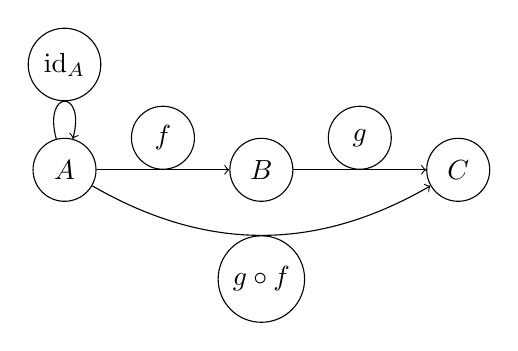
\begin{tikzpicture}[node distance=2.5cm, every node/.style={circle, draw, minimum size=0.8cm}]
    \node (A) {$A$};
    \node (B) [right of=A] {$B$};
    \node (C) [right of=B] {$C$};
    \draw[->] (A) to node[above] {$f$} (B);
    \draw[->] (B) to node[above] {$g$} (C);
    \draw[->, bend right=30] (A) to node[below] {$g \circ f$} (C);
    \draw[->] (A) to [loop above] node {$\mathrm{id}_A$} (A);
\end{tikzpicture}
\end{center}

\subsubsection{Formal Definition}

\begin{definition}[Category]
A \textbf{category} $\mathcal{C}$ consists of:
\begin{itemize}
    \item A collection $\mathrm{Ob}(\mathcal{C})$ of \textbf{objects}
    \item For each pair of objects $A, B$, a collection $\mathrm{Hom}(A, B)$ of \textbf{morphisms} from $A$ to $B$
    \item For each object $A$, an \textbf{identity morphism} $\mathrm{id}_A \in \mathrm{Hom}(A, A)$
    \item For each triple $A, B, C$, a \textbf{composition operation}:
    \[ \circ : \mathrm{Hom}(B, C) \times \mathrm{Hom}(A, B) \to \mathrm{Hom}(A, C) \]
\end{itemize}
satisfying:
\begin{enumerate}
    \item \textbf{Associativity:} $(h \circ g) \circ f = h \circ (g \circ f)$

    \textit{``It doesn't matter how you group compositions---the result is the same.''}

    \item \textbf{Identity laws:} $f \circ \mathrm{id}_A = f$ and $\mathrm{id}_B \circ f = f$ for any $f: A \to B$

    \textit{``Composing with identity does nothing.''}
\end{enumerate}
\end{definition}

\subsubsection{Why These Axioms?}

The axioms capture the minimal requirements for ``things and transformations between them'':

\begin{itemize}
    \item \textbf{Associativity} says composition is well-behaved. If you transform $A \to B \to C \to D$, you get the same result whether you first compose $A \to B \to C$ and then go to $D$, or first compose $B \to C \to D$ and apply $A$ to that. No ambiguity.

    \item \textbf{Identity} says every object has a trivial ``self-transformation.'' This is like the number $0$ for addition or $1$ for multiplication---it's the ``do nothing'' operation.
\end{itemize}

\begin{example}[Some categories]\leavevmode
\begin{itemize}
    \item $\mathbf{Set}$: objects are sets, morphisms are functions, composition is function composition, identity is the identity function $x \mapsto x$.

    \item $\mathbf{Grp}$: objects are groups, morphisms are group homomorphisms (functions that preserve the group operation), composition and identity as in $\mathbf{Set}$.

    \item $\mathbf{Top}$: objects are topological spaces, morphisms are continuous maps.

    \item $\mathbf{Pos}$: objects are partially ordered sets, morphisms are monotone functions ($x \leq y \Rightarrow f(x) \leq f(y)$).

    \item $\mathbf{Vect}_k$: objects are vector spaces over field $k$, morphisms are linear maps.
\end{itemize}
\end{example}

\begin{intuition}
Notice the pattern: in each case, morphisms are ``structure-respecting maps.'' Functions respect set structure (elements map to elements). Homomorphisms respect group structure ($f(ab) = f(a)f(b)$). Continuous maps respect topological structure (preimages of open sets are open).

A category isolates this pattern: objects have some structure, morphisms respect it. We can then study properties that depend only on this pattern, not on the specific structures involved.
\end{intuition}

\begin{keyinsight}
Category theory is the \textbf{mathematics of mathematics}. It studies structure and invariance in full generality.

This is exactly what logic needed: a language where \emph{transformations} and \emph{what they preserve} are first-class concepts.
\end{keyinsight}

\section{Lawvere: Logic Meets Category Theory}

In the 1960s, F. William Lawvere showed that logic itself could be expressed categorically.

\begin{history}
Lawvere's thesis (1963) and subsequent work reformulated:
\begin{itemize}
    \item Theories as categories
    \item Models as functors
    \item Logical operations as categorical constructions (products, exponentials, etc.)
\end{itemize}
\end{history}

Let's unpack what this means.

\subsubsection{Conjunction is Product}

In logic, $A \land B$ is true when both $A$ and $B$ are true. To have evidence for $A \land B$, you need evidence for $A$ \emph{and} evidence for $B$.

In category theory, this is exactly a \textbf{product} $A \times B$: an object equipped with projections to both $A$ and $B$, universal among such objects.

\begin{center}
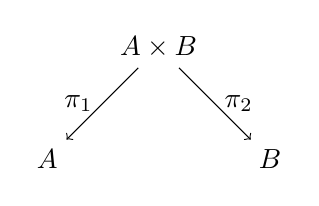
\begin{tikzpicture}[node distance=2cm]
    \node (AB) {$A \times B$};
    \node (A) [below left of=AB] {$A$};
    \node (B) [below right of=AB] {$B$};
    \draw[->] (AB) -- node[left] {$\pi_1$} (A);
    \draw[->] (AB) -- node[right] {$\pi_2$} (B);
\end{tikzpicture}
\end{center}

\textit{Having a proof of $A \land B$ means having a pair: a proof of $A$ and a proof of $B$.}

\subsubsection{Disjunction is Coproduct}

In logic, $A \lor B$ is true when at least one of $A$ or $B$ is true.

In category theory, this is a \textbf{coproduct} (or sum) $A + B$: an object with injections from both $A$ and $B$.

\textit{A proof of $A \lor B$ is either a proof of $A$ or a proof of $B$ (tagged with which one).}

\subsubsection{Implication is Exponential}

This is deeper. In logic, $A \to B$ means ``if $A$ then $B$.'' A proof of $A \to B$ is a \emph{method} that transforms any proof of $A$ into a proof of $B$.

In category theory, this is the \textbf{exponential object} $B^A$ (also written $[A, B]$ or $A \Rightarrow B$).

\begin{definition}[Exponential Object]
In a category, the \textbf{exponential} $B^A$ is an object representing ``morphisms from $A$ to $B$.'' It is characterized by a natural bijection:
\[
\mathrm{Hom}(C \times A, B) \;\cong\; \mathrm{Hom}(C, B^A)
\]
\end{definition}

What does this mean? Let's translate:

\textbf{Left side:} Maps from $C \times A$ to $B$. These are functions that take a pair $(c, a)$ and produce a $b$.

\textbf{Right side:} Maps from $C$ to $B^A$. These are functions that take a $c$ and produce a ``function from $A$ to $B$.''

The bijection says: a function of two arguments is the same as a function that returns a function. This is \textbf{currying}!

\begin{example}[In $\mathbf{Set}$]
In the category of sets, $B^A$ is exactly the set of all functions from $A$ to $B$:
\[ B^A = \{ f : A \to B \} \]
The bijection is currying:
\[ f(c, a) = b \quad\longleftrightarrow\quad g(c) = (\lambda a.\, f(c, a)) \]
\end{example}

\textit{Why the notation $B^A$? Because $|B^A| = |B|^{|A|}$---if $B$ has $m$ elements and $A$ has $n$ elements, there are $m^n$ functions from $A$ to $B$.}

\subsubsection{Quantifiers are Adjoints}

Now for the deepest part: quantifiers as adjoints.

First, what is an \textbf{adjunction}? Informally, two functors $F$ and $G$ are adjoint if they're ``almost inverses'' in a specific sense:

\begin{definition}[Adjunction, informally]
$F : \mathcal{C} \to \mathcal{D}$ is \textbf{left adjoint} to $G : \mathcal{D} \to \mathcal{C}$ (written $F \dashv G$) if there's a natural bijection:
\[
\mathrm{Hom}_{\mathcal{D}}(F(A), B) \;\cong\; \mathrm{Hom}_{\mathcal{C}}(A, G(B))
\]
\end{definition}

\textit{``A map out of $F(A)$ is the same as a map into $G(B)$.'' $F$ and $G$ are two perspectives on the same relationship.}

Now, how do quantifiers fit in?

Consider a projection $\pi : A \times B \to A$ (forgetting the $B$ component). This induces a functor $\pi^* : \mathbf{Set}/A \to \mathbf{Set}/(A \times B)$ that pulls back predicates.

\begin{itemize}
    \item \textbf{Existential quantifier $\exists$} is the \textbf{left adjoint} to pullback.

    \textit{``There exists a $b$ such that $P(a, b)$'' collapses the $B$-dimension by asking ``is there at least one?''}

    \item \textbf{Universal quantifier $\forall$} is the \textbf{right adjoint} to pullback.

    \textit{``For all $b$, $P(a, b)$'' collapses the $B$-dimension by asking ``does it hold for every one?''}
\end{itemize}

\begin{intuition}
Why adjoints? Because $\exists$ and $\forall$ satisfy these bijections:

\textbf{For $\exists$:} To prove $(\exists b.\, P(a,b)) \to Q(a)$, it suffices to prove $P(a,b) \to Q(a)$ (for arbitrary $b$). If $Q$ holds whenever $P$ holds for any specific $b$, then $Q$ holds when $P$ holds for \emph{some} $b$.

\textbf{For $\forall$:} To prove $Q(a) \to (\forall b.\, P(a,b))$, you must prove $Q(a) \to P(a,b)$ for each $b$. If from $Q$ you can derive $P$ for any specific $b$, then from $Q$ you can derive $P$ for \emph{all} $b$.

These are exactly the adjunction bijections in disguise!
\end{intuition}

\begin{keyinsight}
The duality between $\exists$ (left adjoint) and $\forall$ (right adjoint) is not a coincidence---it's the same duality that appears throughout mathematics:
\begin{itemize}
    \item Free structures (left adjoint) vs. forgetful functors (right adjoint)
    \item Tensor product (left adjoint) vs. Hom (right adjoint)
    \item Image (left adjoint) vs. preimage (right adjoint)
\end{itemize}
Quantifiers are just another instance of this universal pattern.
\end{keyinsight}

This is not just a translation. It reveals the \textbf{structural essence} of logic, stripped of the accidents of set-theoretic encoding. Implication, conjunction, disjunction, quantification---all emerge from categorical structure.

\section{Topos Theory: Logic and Geometry Unite}

Lawvere and Myles Tierney developed \textbf{topos theory}: categories that behave like the category of sets, but with an internal logic that can differ from classical logic.

\begin{intuition}
A topos is a ``universe of mathematics'' with its own internal logic. Different toposes can have different logics: classical, intuitionistic, or even more exotic.

This unified logic and geometry: a topos is both a geometric object (like a space) and a logical universe (where you can do mathematics).
\end{intuition}

\section{Algebra and Coalgebra: Two Faces of Structure}

Within category theory, a fundamental duality emerged: \textbf{algebra} and \textbf{coalgebra}.

\subsection{Algebra: Building Up}

An \textbf{algebra} for a functor $F$ is a structure where you can ``fold'' or ``evaluate'' $F$-structured data.

\begin{example}[Lists as an algebra]
The type of lists of natural numbers satisfies:
\[
\mathsf{List}(\mathbb{N}) \cong 1 + \mathbb{N} \times \mathsf{List}(\mathbb{N})
\]
A list is either empty ($1$) or a head ($\mathbb{N}$) followed by a tail (another list).

This is an \textbf{algebra} for the functor $F(X) = 1 + \mathbb{N} \times X$.

Functions on lists (like $\mathsf{sum}$) are defined by \textbf{folding}: specify what to do with empty and what to do with cons.
\end{example}

Algebras are about \textbf{construction} and \textbf{induction}: building finite, well-founded structures.

The syntax of a logic---formulas, proofs---forms an algebra: the \textbf{initial algebra} of the grammar.

\subsection{Coalgebra: Observing Behavior}

A \textbf{coalgebra} for a functor $F$ is a structure where you can ``unfold'' or ``observe'' behavior.

\begin{example}[Streams as a coalgebra]
An infinite stream of natural numbers has type:
\[
\mathsf{Stream}(\mathbb{N}) \to \mathbb{N} \times \mathsf{Stream}(\mathbb{N})
\]
From a stream, you can observe: the head (a number) and the tail (another stream).

This is a \textbf{coalgebra} for the functor $F(X) = \mathbb{N} \times X$.

Functions producing streams are defined by \textbf{unfolding}: specify the head and how to continue.
\end{example}

Coalgebras are about \textbf{behavior} and \textbf{coinduction}: potentially infinite, observable processes.

State machines, automata, transition systems---these are coalgebras.

\subsection{The Duality}

\begin{center}
\begin{tabular}{lll}
& \textbf{Algebra} & \textbf{Coalgebra} \\
\hline
Perspective & Construction & Observation \\
Principle & Induction & Coinduction \\
Structure & Finite, well-founded & Potentially infinite \\
Examples & Syntax, data types & Behavior, state machines \\
Canonical object & Initial algebra & Final coalgebra \\
\end{tabular}
\end{center}

\begin{keyinsight}
Algebra is about \textbf{syntax}: how things are built.\\
Coalgebra is about \textbf{semantics}: how things behave.

Logic lives in both: the formulas are algebraic (syntax), but their meaning involves coalgebraic structures (models, possible worlds, state transitions).
\end{keyinsight}

\section{Modal Logic as Coalgebraic Logic}

Here is where everything connects.

Remember Kripke semantics for modal logic? A \textbf{Kripke frame} is a pair $(W, R)$ where:
\begin{itemize}
    \item $W$ is a set of ``possible worlds''
    \item $R \subseteq W \times W$ is an ``accessibility relation''
\end{itemize}

But this is exactly a \textbf{coalgebra}! A Kripke frame is a coalgebra for the powerset functor:
\[
\alpha: W \to \mathcal{P}(W)
\]
where $\alpha(w) = \{v \mid w R v\}$---the set of worlds accessible from $w$.

\begin{keyinsight}
\textbf{Kripke frames are coalgebras.}

And the key notion of equivalence for coalgebras is \textbf{bisimulation}---which is exactly the right notion of equivalence for modal logic!

Van Benthem's theorem: modal logic is the \textbf{bisimulation-invariant} fragment of first-order logic.
\end{keyinsight}

This is not a coincidence. Modal logic is the \textbf{natural language for describing coalgebraic behavior}.

Different modal logics arise from different functors:
\begin{itemize}
    \item Kripke frames: $F(X) = \mathcal{P}(X)$
    \item Labeled transition systems: $F(X) = \mathcal{P}(A \times X)$ for action set $A$
    \item Probabilistic systems: $F(X) = \mathcal{D}(X)$ (probability distributions)
    \item Automata: $F(X) = 2 \times X^A$ (accepting/rejecting + transitions)
\end{itemize}

\textbf{Coalgebraic modal logic} provides a uniform treatment of all these cases.

\section{The Modern Landscape}

Let us step back and see where we are.

\begin{center}
\begin{tikzpicture}[node distance=2cm, auto]
    \node (form) {\textbf{``Form + Structure-preserving''}};
    \node (four) [below=1.5cm of form] {Four Pillars};
    \node (cat) [below=1.5cm of four] {Category Theory};
    \node (alg) [below left=1.5cm and 1cm of cat] {Algebra (Syntax)};
    \node (coalg) [below right=1.5cm and 1cm of cat] {Coalgebra (Behavior)};
    \node (modal) [below=1.5cm of coalg] {Modal Logic};

    \draw[->] (form) -- (four) node[midway, right] {\small 20th century};
    \draw[->] (four) -- (cat) node[midway, right] {\small ``what is structure?''};
    \draw[->] (cat) -- (alg);
    \draw[->] (cat) -- (coalg);
    \draw[->] (coalg) -- (modal) node[midway, right] {\small natural language for};
\end{tikzpicture}
\end{center}

The journey, driven throughout by the desire for greater expressive power:
\begin{enumerate}
    \item \textbf{Syllogisms}: ``I want to describe valid argument forms''
    \item \textbf{First-order logic}: ``I want to describe quantified relationships''
    \item \textbf{Modal logic}: ``I want to describe possibility, necessity, time, knowledge...''
    \item \textbf{The shift}: Logic becomes a language for describing systems, not just a tool for checking arguments
    \item \textbf{Category theory}: ``I want to describe structure itself''
    \item \textbf{Algebra/Coalgebra}: Syntax vs. behavior---two faces of structure
    \item \textbf{Coalgebraic modal logic}: Modal logic is the natural language for behavioral systems
\end{enumerate}

Each step: \emph{I can't say what I want to say} $\to$ \emph{build a more expressive language}.

\section{Why This Matters for Us}

This book is about \textbf{the algebra of intelligence}. We want to understand:
\begin{itemize}
    \item How can agents reason about possibility, knowledge, change?
    \item How can we specify and verify agent behavior?
    \item How can formal structures \emph{learn}?
\end{itemize}

Modal logic gives us the \textbf{language}.

Coalgebra gives us the \textbf{semantics}---a unified framework for all kinds of state-based, behavioral systems.

And the algebraic/coalgebraic duality will be crucial when we ask: how do we make these structures \textbf{learnable}?

But first, we need to understand modal logic properly. That begins in the next chapter, with Kripke frames.

\begin{summary}
The history of logic is the history of the desire for greater expressive power.

\begin{itemize}
    \item \textbf{The ladder}: syllogisms $\to$ propositional $\to$ first-order $\to$ modal $\to$ ...
    \item \textbf{The shift}: from ``studying consequence'' to ``describing structured systems''
    \item \textbf{The convergence}: philosophers, linguists, computer scientists all need to describe systems
    \item \textbf{The ultimate abstraction}: category theory---the language of structure itself
    \item \textbf{The duality}: algebra (syntax, construction) vs. coalgebra (behavior, observation)
    \item \textbf{The connection}: modal logic is the natural language for coalgebraic systems
\end{itemize}

One thread runs through it all: \emph{I can't say what I want to say---so I build a more expressive language.}
\end{summary}
